\chapter{Descripción del problema}

\textit{DYNAsystem} aspira a ser un dispositivo utilizado tanto por deportistas como por investigadores de ciencias de la salud y preparadores físicos de todo el mundo; para lo que la compañía se enfoca a tres distintas líneas de mercado: \texttt{\textit{HEALTH}} (salud), \texttt{\textit{SPORT}} (deporte) y \texttt{\textit{RESEARCH}} (investigación). Sin embargo, para llegar a estas cotas de mercado ha de ser un \textbf{sistema funcional, versátil, único e innovador}.\\

\begin{figure}[H]
	\centering
	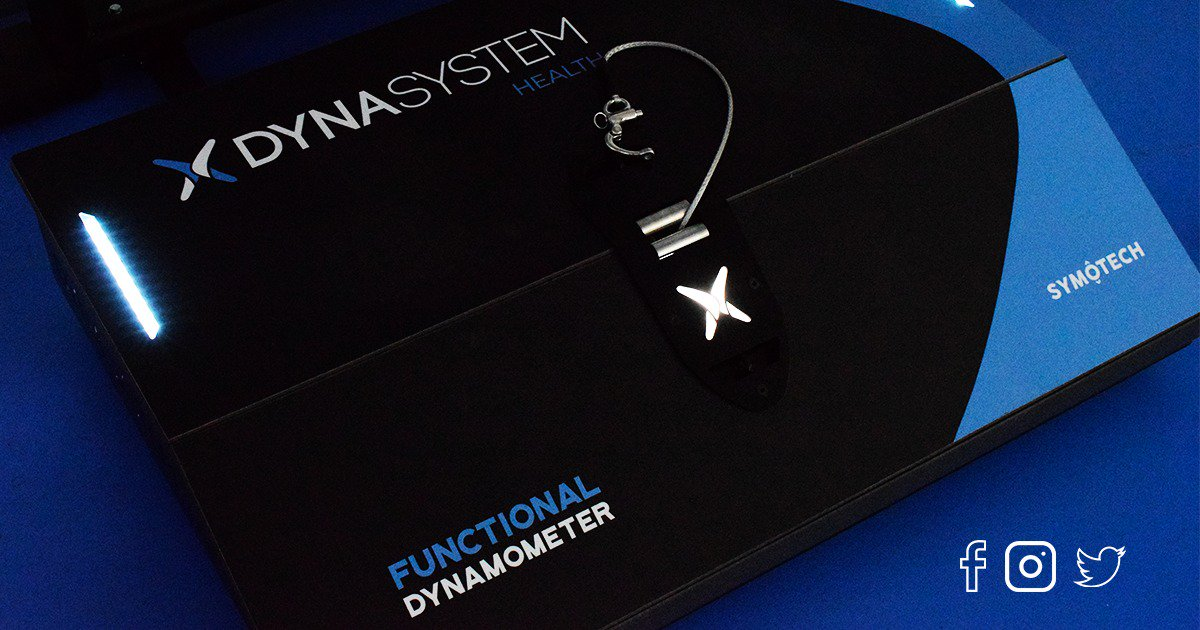
\includegraphics[width=0.7\linewidth]{imagenes/dynasystem-blue-floor.jpeg}
	\caption{Dispositivo \textit{DYNAsystem}, de la línea \textbf{\textit{HEALTH}} - \href{https://twitter.com/dynasystem_/status/1001762762111021057}{\textit{Tweet} promocional del producto} [30/05/2018]}
	\label{dynasystem-health}
\end{figure}

Mientras que la apariencia estética será la primera impresión que tendrá del producto un potencial cliente, es necesario que tanto la electrónica interna como el \textit{software embebido} cumplan con su cometido y animen al usuario a seguir utilizando la máquina. Para ello, es de vital importancia que este re-diseño solucione errores de los dispositivos antiguos que comentamos en el apartado anterior, como lo son la \textbf{inestabilidad} (producida quizás por reinicios y/o bloqueos inesperados), la \textbf{latencia} (entendiéndose ésta como retardo en el arranque o la usabilidad) y la \textbf{falta de medios para depuración de errores} (como la ausencia de una consola de administración, o la posibilidad de actualizar remotamente las máquinas vía software). Veamos de forma más directa la descripción del problema, desde un punto de vista funcional y del producto (sin entrar en demasiados detalles técnicos o estructurales), en contraposición con las máquinas antiguas (previamente mencionadas):\\

El dispositivo antecedente a éste se demoraba demasiado en el arranque, inicializando interfaces de red y cargando en memoria la aplicación. Sin embargo, para un caso de éxito, la máquina ha de estar lista para empezar a trabajar con ella lo antes posible desde que se accione su interruptor. Cuanto menos tiempo espere el usuario para configurar su ejercicio, mejor impresión tendrá del producto. Por tanto, es de vital importancia que además de disponer de una infraestructura rápida y ligera, el usuario no tenga que pasar por una pantalla de inicio de sesión como habría de hacerlo en un ordenador convencional.\\

Lógicamente, será necesario que la infraestructura ejecute la aplicación antes mencionada, en torno a la que gira el sistema. Por lo que ésta sufre algún problema o cierre inesperado, el sistema habrá de restaurar su estado (reiniciando automáticamente si la ocasión lo requiere), ya que si el programa no está corriendo, no tendrá sentido que el dispositivo esté en funcionamiento.\\

Durante el tiempo de encendido, el usuario no querrá que su innovador dispositivo le muestre en pantalla una ventana negra de comandos con texto en blanco, por ejemplo, mostrando mensajes del \textit{kernel} de \textit{Linux} en carga. Preferiblemente, le gustará ver algún tipo de imagen estática o animada durante el proceso, que desaparezca con dicha aplicación ya preparada.\\

El sistema deberá permitir la conexión a Internet, de forma tanto inalámbrica como cableada, de forma transparente e intuitiva para el usuario. En un futuro se espera tener aplicaciones móviles capaces de tratar los datos emitidos por la máquina, por lo que esta necesidad de conectividad es imperativa.\\

Se espera que se puedan guardar datos brutos generados por la aplicación en un dispositivo de almacenamiento externo (como por ejemplo un \textit{pendrive} o un disco duro convencional).\\

Una de las carencias que sufría el dispositivo implementado por la compañía antigua era la falta de medios de depuración de fallos de software surgidos a lo largo del tiempo. Por tanto, se requiere disponer de un sistema de actualizaciones integrado con el dispositivo que permita solucionarlos de forma remota, ahorrando grandes costes en movilización de servicio técnico.\\

Este protocolo de actualización podrá hacerse mediante red cableada o \textit{Wi-Fi} (dadas las especificaciones de conectividad de la máquina), y deberá ser lo suficientemente inteligente para saber cuándo una actualización ha sido instalada con éxito; asegurándose de que todo ha ido según lo esperado y retornando a la versión anterior si la nueva impidiese el uso o dejase al dispositivo incomunicado. Por otro lado, dicho sistema de actualizaciones deberá pedir confirmación al usuario antes de aplicar las nuevas instalaciones, de forma que no lo interrumpan en sus ejercicios.\\

El proceso de actualización debe ser fácilmente implementable y llevado a cabo de forma sencilla por una pequeña parte del equipo de desarrollo, que registren los cambios de versiones y desplieguen las actualizaciones desde sus puestos de trabajo.\\

Aunque se espera que el dispositivo tenga diversas formas de administración y/o recuperación, por \textbf{seguridad} es necesario que la entrada de teclado no sea una de ellas; ya que cualquier usuario curioso podría utilizarlo para cerrar la aplicación y manipular el sistema operativo con resultados inesperados.\\

\newpage